\documentclass[oneside]{ctexbook}
\usepackage{minted}
\usepackage{tikz}
\usepackage{amsmath}

\usepackage{xcolor} % to access the named colour LightGray
\definecolor{LightGray}{gray}{0.9}

\setminted[java]{
    frame=lines,
    linenos,
    breaklines,
    bgcolor=LightGray,
    fontsize=\footnotesize,
    framesep=2mm,
    escapeinside=||,
    mathescape=true
}

\title{LeetCode刷题指南}
\author{左元}

\begin{document}

\maketitle
\tableofcontents

\begin{quote}
    过早优化是万恶之源. -高德纳
\end{quote}

\chapter{两数之和}

\section{题目}

给定一个整数数组nums和一个整数目标值target, 请你在该数组中找出和为目标值target的那两个整数, 并返回它们的数组下标.

你可以假设每种输入只会对应一个答案. 但是, 数组中同一个元素在答案里不能重复出现.

你可以按任意顺序返回答案.

\textbf{示例 1}:

\begin{minted}{text}
输入: nums = [2,7,11,15], target = 9
输出: [0,1]
解释: 因为 nums[0] + nums[1] == 9, 返回 [0, 1].
\end{minted}

\textbf{示例 2}:

\begin{minted}{text}
输入: nums = [3,2,4], target = 6
\end{minted}

\textbf{示例 3}:

\begin{minted}{text}
输入: nums = [3,3], target = 6
输出: [0,1]
\end{minted}

\textbf{提示}:

\begin{itemize}
  \item $2 <= nums.length <= 10^4$
  \item $-10^9 <= nums[i] <= 10^9$
  \item $-10^9 <= target <= 10^9$
  \item 只会存在一个有效答案
\end{itemize}

\textbf{进阶}: 你可以想出一个时间复杂度小于 $O(n^2)$ 的算法吗?

\section{解法}

\subsection{暴力法}

\tikzset{every picture/.style={line width=0.75pt}} %set default line width to 0.75pt        

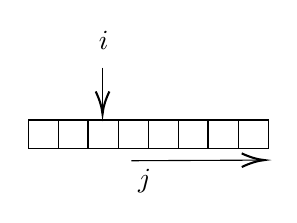
\begin{tikzpicture}[x=0.75pt,y=0.75pt,yscale=-1,xscale=1]
%uncomment if require: \path (0,300); %set diagram left start at 0, and has height of 300

%Shape: Rectangle [id:dp3457694059016647] 
\draw   (106,47.8) -- (120.6,47.8) -- (120.6,61.6) -- (106,61.6) -- cycle ;
%Shape: Rectangle [id:dp7301709212004892] 
\draw   (120.6,47.8) -- (135.2,47.8) -- (135.2,61.6) -- (120.6,61.6) -- cycle ;
%Shape: Rectangle [id:dp6002083473163116] 
\draw   (134.8,47.8) -- (149.4,47.8) -- (149.4,61.6) -- (134.8,61.6) -- cycle ;
%Shape: Rectangle [id:dp08397594893702254] 
\draw   (149.4,47.8) -- (164,47.8) -- (164,61.6) -- (149.4,61.6) -- cycle ;
%Shape: Rectangle [id:dp08205591010512414] 
\draw   (163.8,47.8) -- (178.4,47.8) -- (178.4,61.6) -- (163.8,61.6) -- cycle ;
%Shape: Rectangle [id:dp9175762103953684] 
\draw   (178.4,47.8) -- (193,47.8) -- (193,61.6) -- (178.4,61.6) -- cycle ;
%Shape: Rectangle [id:dp9418675044381374] 
\draw   (192.6,47.8) -- (207.2,47.8) -- (207.2,61.6) -- (192.6,61.6) -- cycle ;
%Shape: Rectangle [id:dp6618380440075453] 
\draw   (207.2,47.8) -- (221.8,47.8) -- (221.8,61.6) -- (207.2,61.6) -- cycle ;
%Straight Lines [id:da5938212204406471] 
\draw    (141.8,22.6) -- (141.8,43) ;
\draw [shift={(141.8,45)}, rotate = 270] [color={rgb, 255:red, 0; green, 0; blue, 0 }  ][line width=0.75]    (10.93,-3.29) .. controls (6.95,-1.4) and (3.31,-0.3) .. (0,0) .. controls (3.31,0.3) and (6.95,1.4) .. (10.93,3.29)   ;
%Straight Lines [id:da1079690828843366] 
\draw    (155.67,67.44) -- (217.8,67.14) ;
\draw [shift={(219.8,67.13)}, rotate = 179.72] [color={rgb, 255:red, 0; green, 0; blue, 0 }  ][line width=0.75]    (10.93,-3.29) .. controls (6.95,-1.4) and (3.31,-0.3) .. (0,0) .. controls (3.31,0.3) and (6.95,1.4) .. (10.93,3.29)   ;

% Text Node
\draw (138.8,3.6) node [anchor=north west][inner sep=0.75pt]   [align=left] {$\displaystyle i$};
% Text Node
\draw (157.67,70.44) node [anchor=north west][inner sep=0.75pt]   [align=left] {$\displaystyle j$};

\end{tikzpicture}

如图所示, $i$ 为当前遍历到的元素, 然后从 $i+1$ 也就是 $j$ 的初始值开始往后寻找和第 $i$ 个元素相加等于target的元素.

\begin{minted}{java}
class Solution {
    public int[] twoSum(int[] nums, int target) {
        // 因为循环的存在, 以下时间复杂度可以忽略.
        int[] result = new int[2]; // $O(1)$

        // 外层循环最多是 $N$ 次
        for (int i = 0; i < nums.length; i++) {
            // 内存循环最多 $N - i - 1$ 次
            for (int j = i + 1; j < nums.length; j++) {
                // 以下几行的时间复杂度可以近似为 $O(1)$
                if (nums[i] + nums[j] == target) { // $O(1)$
                    result[0] = i; // $O(1)$
                    result[1] = j; // $O(1)$
                    return result; // $O(1)$
                }
            }
        }

        // 因为循环的存在, 以下时间复杂度可以忽略.
        return null; // $O(1)$
    }
}
\end{minted}

所以时间复杂度的计算过程如下:

\begin{equation*}
    \begin{split}
    T(N) &= O(N-0-1) + O(N-1-1) + ... + O(N-(N-1)-1) \\
         &= O(N-1) + O(N-2) + ... + O(0) \\
         &= O(\frac{N-1}{2}) \\
         &\approx O(N^2)
    \end{split}
\end{equation*}

\subsection{哈希法}

暴力解法的问题是时间复杂度是 $O(N^2)$. 所以我们需要把时间复杂度降下来. 这里考虑使用哈希表来解决这个问题.

哈希表的key是\textbf{数组元素}.

哈希表的value是\textbf{数组元素的索引}.

每遍历一个数组元素, 就在哈希表中查看一下是否有某个key和当前遍历的数组元素相加为target. 如果有, 那么直接返回. 如果没有, 那么将当前遍历的数组元素作为key, 索引作为value, 插入到哈希表中.


\begin{table}[!h]
\centering
    
\begin{tabular}{|p{0.50\textwidth}|p{0.50\textwidth}|}
\hline 
数组元素 & 数组元素的索引 \\
\hline 
3 & 0 \\
\hline 
2 & 1 \\
\hline 
4 & 2 \\
\hline
\end{tabular}
    
\end{table}

\begin{minted}[escapeinside=||,mathescape=true,linenos]{java}
class Solution {
    public int[] twoSum(int[] nums, int target) {
        var result = new int[2];

        var map = new HashMap<Integer, Integer>();
        // 循环次数最多是 $O(N)$ 次.
        for (int i = 0; i < nums.length; i++) {
            // 以下条件语句的时间复杂度可以近似为 $O(1)$
            if (map.get(target - nums[i]) != null) {
                result[0] = i;
                result[1] = map.get(target - nums[i]);
                return result;
            } else {
                map.put(nums[i], i);
            }
        }

        return null;
    }
}
\end{minted}

所以时间复杂度是 $O(N)$.

\chapter{两数相加}

\section{题目}

给你两个\textbf{非空}的链表, 表示两个非负的整数. 它们每位数字都是按照\textbf{逆序}的方式存储的, 并且每个节点只能存储\textbf{一位}数字.

请你将两个数相加, 并以相同形式返回一个表示和的链表.

你可以假设除了数字 0 之外, 这两个数都不会以 0 开头.

\textbf{示例 1}:



\tikzset{every picture/.style={line width=0.75pt}} %set default line width to 0.75pt        

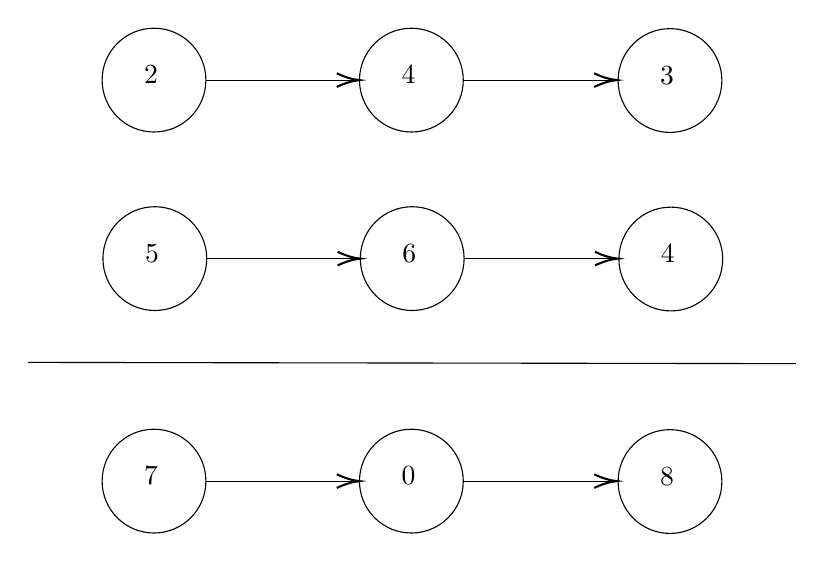
\begin{tikzpicture}[x=0.75pt,y=0.75pt,yscale=-1,xscale=1]
%uncomment if require: \path (0,300); %set diagram left start at 0, and has height of 300

%Shape: Circle [id:dp7818164950316125] 
\draw   (96,60) .. controls (96,46.19) and (107.19,35) .. (121,35) .. controls (134.81,35) and (146,46.19) .. (146,60) .. controls (146,73.81) and (134.81,85) .. (121,85) .. controls (107.19,85) and (96,73.81) .. (96,60) -- cycle ;
%Shape: Circle [id:dp2630950889358923] 
\draw   (220,60) .. controls (220,46.19) and (231.19,35) .. (245,35) .. controls (258.81,35) and (270,46.19) .. (270,60) .. controls (270,73.81) and (258.81,85) .. (245,85) .. controls (231.19,85) and (220,73.81) .. (220,60) -- cycle ;
%Shape: Circle [id:dp7516794003180826] 
\draw   (344.6,60.2) .. controls (344.6,46.39) and (355.79,35.2) .. (369.6,35.2) .. controls (383.41,35.2) and (394.6,46.39) .. (394.6,60.2) .. controls (394.6,74.01) and (383.41,85.2) .. (369.6,85.2) .. controls (355.79,85.2) and (344.6,74.01) .. (344.6,60.2) -- cycle ;
%Straight Lines [id:da7245742761900981] 
\draw    (146,60) -- (218,60) ;
\draw [shift={(220,60)}, rotate = 180] [color={rgb, 255:red, 0; green, 0; blue, 0 }  ][line width=0.75]    (10.93,-3.29) .. controls (6.95,-1.4) and (3.31,-0.3) .. (0,0) .. controls (3.31,0.3) and (6.95,1.4) .. (10.93,3.29)   ;
%Straight Lines [id:da4623332980145326] 
\draw    (270,60) -- (342,60) ;
\draw [shift={(344,60)}, rotate = 180] [color={rgb, 255:red, 0; green, 0; blue, 0 }  ][line width=0.75]    (10.93,-3.29) .. controls (6.95,-1.4) and (3.31,-0.3) .. (0,0) .. controls (3.31,0.3) and (6.95,1.4) .. (10.93,3.29)   ;
%Shape: Circle [id:dp9405952440212225] 
\draw   (96.4,146) .. controls (96.4,132.19) and (107.59,121) .. (121.4,121) .. controls (135.21,121) and (146.4,132.19) .. (146.4,146) .. controls (146.4,159.81) and (135.21,171) .. (121.4,171) .. controls (107.59,171) and (96.4,159.81) .. (96.4,146) -- cycle ;
%Shape: Circle [id:dp511626874279288] 
\draw   (220.4,146) .. controls (220.4,132.19) and (231.59,121) .. (245.4,121) .. controls (259.21,121) and (270.4,132.19) .. (270.4,146) .. controls (270.4,159.81) and (259.21,171) .. (245.4,171) .. controls (231.59,171) and (220.4,159.81) .. (220.4,146) -- cycle ;
%Shape: Circle [id:dp7434931354800127] 
\draw   (345,146.2) .. controls (345,132.39) and (356.19,121.2) .. (370,121.2) .. controls (383.81,121.2) and (395,132.39) .. (395,146.2) .. controls (395,160.01) and (383.81,171.2) .. (370,171.2) .. controls (356.19,171.2) and (345,160.01) .. (345,146.2) -- cycle ;
%Straight Lines [id:da9351749080021932] 
\draw    (146.4,146) -- (218.4,146) ;
\draw [shift={(220.4,146)}, rotate = 180] [color={rgb, 255:red, 0; green, 0; blue, 0 }  ][line width=0.75]    (10.93,-3.29) .. controls (6.95,-1.4) and (3.31,-0.3) .. (0,0) .. controls (3.31,0.3) and (6.95,1.4) .. (10.93,3.29)   ;
%Straight Lines [id:da5935525870849152] 
\draw    (270.4,146) -- (342.4,146) ;
\draw [shift={(344.4,146)}, rotate = 180] [color={rgb, 255:red, 0; green, 0; blue, 0 }  ][line width=0.75]    (10.93,-3.29) .. controls (6.95,-1.4) and (3.31,-0.3) .. (0,0) .. controls (3.31,0.3) and (6.95,1.4) .. (10.93,3.29)   ;
%Shape: Circle [id:dp7952381161886958] 
\draw   (96,253.2) .. controls (96,239.39) and (107.19,228.2) .. (121,228.2) .. controls (134.81,228.2) and (146,239.39) .. (146,253.2) .. controls (146,267.01) and (134.81,278.2) .. (121,278.2) .. controls (107.19,278.2) and (96,267.01) .. (96,253.2) -- cycle ;
%Shape: Circle [id:dp16231160678412393] 
\draw   (220,253.2) .. controls (220,239.39) and (231.19,228.2) .. (245,228.2) .. controls (258.81,228.2) and (270,239.39) .. (270,253.2) .. controls (270,267.01) and (258.81,278.2) .. (245,278.2) .. controls (231.19,278.2) and (220,267.01) .. (220,253.2) -- cycle ;
%Shape: Circle [id:dp968034384158754] 
\draw   (344.6,253.4) .. controls (344.6,239.59) and (355.79,228.4) .. (369.6,228.4) .. controls (383.41,228.4) and (394.6,239.59) .. (394.6,253.4) .. controls (394.6,267.21) and (383.41,278.4) .. (369.6,278.4) .. controls (355.79,278.4) and (344.6,267.21) .. (344.6,253.4) -- cycle ;
%Straight Lines [id:da30048639995487847] 
\draw    (146,253.2) -- (218,253.2) ;
\draw [shift={(220,253.2)}, rotate = 180] [color={rgb, 255:red, 0; green, 0; blue, 0 }  ][line width=0.75]    (10.93,-3.29) .. controls (6.95,-1.4) and (3.31,-0.3) .. (0,0) .. controls (3.31,0.3) and (6.95,1.4) .. (10.93,3.29)   ;
%Straight Lines [id:da3148946678405248] 
\draw    (270,253.2) -- (342,253.2) ;
\draw [shift={(344,253.2)}, rotate = 180] [color={rgb, 255:red, 0; green, 0; blue, 0 }  ][line width=0.75]    (10.93,-3.29) .. controls (6.95,-1.4) and (3.31,-0.3) .. (0,0) .. controls (3.31,0.3) and (6.95,1.4) .. (10.93,3.29)   ;
%Straight Lines [id:da6161416091999112] 
\draw    (60.4,196) -- (430.2,196.6) ;

% Text Node
\draw (115,52) node [anchor=north west][inner sep=0.75pt]   [align=left] {2};
% Text Node
\draw (239,52) node [anchor=north west][inner sep=0.75pt]   [align=left] {4};
% Text Node
\draw (363.6,52.2) node [anchor=north west][inner sep=0.75pt]   [align=left] {3};
% Text Node
\draw (115.4,138) node [anchor=north west][inner sep=0.75pt]   [align=left] {5};
% Text Node
\draw (239.4,138) node [anchor=north west][inner sep=0.75pt]   [align=left] {6};
% Text Node
\draw (364,138.2) node [anchor=north west][inner sep=0.75pt]   [align=left] {4};
% Text Node
\draw (115,245.2) node [anchor=north west][inner sep=0.75pt]   [align=left] {7};
% Text Node
\draw (239,245.2) node [anchor=north west][inner sep=0.75pt]   [align=left] {0};
% Text Node
\draw (363.6,245.4) node [anchor=north west][inner sep=0.75pt]   [align=left] {8};


\end{tikzpicture}


\begin{minted}{text}
输入: l1 = [2,4,3], l2 = [5,6,4]
输出: [7,0,8]
解释: 342 + 465 = 807.
\end{minted}

\textbf{示例 2}:

\begin{minted}{text}
输入: l1 = [0], l2 = [0]
输出: [0]
\end{minted}

\textbf{示例 3}:

\begin{minted}{text}
输入: l1 = [9,9,9,9,9,9,9], l2 = [9,9,9,9]
输出: [8,9,9,9,0,0,0,1]
\end{minted}

\textbf{提示}:

\begin{itemize}
  \item 每个链表中的节点数在范围 [1, 100] 内
  \item 0 <= Node.val <= 9
  \item 题目数据保证列表表示的数字不含前导零
\end{itemize}

\section{链表基础知识}

链表的内存布局. 局部性不够好.

\section{解法}

\begin{minted}{java}
/**
 * Definition for singly-linked list.
 * public class ListNode {
 *     int val;
 *     ListNode next;
 *     ListNode() {}
 *     ListNode(int val) { this.val = val; }
 *     ListNode(int val, ListNode next) { this.val = val; this.next = next; }
 * }
 */
class Solution {
    public ListNode addTwoNumbers(ListNode l1, ListNode l2) {
        var head1 = l1;
        var head2 = l2;

        int flag = 0;

        var dummy = new ListNode(-1);
        var tmp = dummy;

        while (head1 != null && head2 != null) {
            var value = head1.val + head2.val + flag;
            if (value < 10) {
                flag = 0;
            } else {
                value = value % 10;
                flag = 1;
            }

            tmp.next = new ListNode(value);
            tmp = tmp.next;

            head1 = head1.next;
            head2 = head2.next;
        }

        if (head1 != null) {
            while (head1 != null) {
                var value = head1.val + flag;
                if (value < 10) {
                    flag = 0;
                } else {
                    value = value % 10;
                    flag = 1;
                }

                tmp.next = new ListNode(value);
                tmp = tmp.next;

                head1 = head1.next;
            }
        }

        if (head2 != null) {
            while (head2 != null) {
                var value = head2.val + flag;
                if (value < 10) {
                    flag = 0;
                } else {
                    value = value % 10;
                    flag = 1;
                }

                tmp.next = new ListNode(value);
                tmp = tmp.next;

                head2 = head2.next;
            }
        }

        if (flag == 1) {
            tmp.next = new ListNode(1);
        }


        return dummy.next;
    }
}
\end{minted}

以上代码比较容易理解, 但重复代码有点多, 所以简化一下.

\begin{minted}{java}
/**
 * Definition for singly-linked list.
 * public class ListNode {
 *     int val;
 *     ListNode next;
 *     ListNode() {}
 *     ListNode(int val) { this.val = val; }
 *     ListNode(int val, ListNode next) { this.val = val; this.next = next; }
 * }
 */
class Solution {
    public ListNode addTwoNumbers(ListNode l1, ListNode l2) {
        var head1 = l1;
        var head2 = l2;

        int flag = 0;

        var dummy = new ListNode(-1);
        var tmp = dummy;

        while (head1 != null || head2 != null) {
            int v1 = 0;
            int v2 = 0;
            if (head1 != null) v1 = head1.val;
            if (head2 != null) v2 = head2.val;
            var value = v1 + v2 + flag;
            if (value < 10) {
                flag = 0;
            } else {
                value = value % 10;
                flag = 1;
            }

            tmp.next = new ListNode(value);
            tmp = tmp.next;

            if (head1 != null) head1 = head1.next;
            if (head2 != null) head2 = head2.next;
        }

        if (flag == 1) {
            tmp.next = new ListNode(1);
        }


        return dummy.next;
    }
}
\end{minted}

\chapter{无重复字符的最长子串}

\section{题目}

给定一个字符串s, 请你找出其中不含有重复字符的\textbf{最长子串}的长度.

\textbf{示例 1}:

\begin{minted}{text}
输入: s = "abcabcbb"
输出: 3 
解释: 因为无重复字符的最长子串是 "abc", 所以其长度为3.
\end{minted}

\textbf{示例 2}:

\begin{minted}{text}
输入: s = "bbbbb"
输出: 1
解释: 因为无重复字符的最长子串是 "b", 所以其长度为1.
\end{minted}

\textbf{示例 3}:

\begin{minted}{text}
输入: s = "pwwkew"
输出: 3
解释: 因为无重复字符的最长子串是"wke", 所以其长度为3.
     请注意, 你的答案必须是 子串 的长度, "pwke"是一个子序列, 不是子串.
\end{minted}

\textbf{提示}:

\begin{itemize}
    \item $0 <= s.length <= 5 * 10^4$
    \item s由英文字母, 数字, 符号和空格组成
\end{itemize}

\section{解法}

\subsection{暴力法}

\begin{minted}{java}
class Solution {
    public int lengthOfLongestSubstring(String s) {
        // 哈希集合,记录每个字符是否出现过
        var charSet = new HashSet<Character>();
        int N = s.length();
        int maxLength = 0;

        for (int i = 0; i < N; i++) {
            charSet.add(s.charAt(i));
            int tmp = 1;
            for (int j = i + 1; j < N && !charSet.contains(s.charAt(j)); j++) {
                charSet.add(s.charAt(j));
                tmp++;
            }
            maxLength = Math.max(maxLength, tmp);
            charSet.clear();
        }

        return maxLength;
    }
}
\end{minted}

\subsection{滑动窗口解法}

这道题的解法我们使用滑动窗口, 也可以认为是双指针法.

左指针指向子串的开始位置, 右指针不断的向右移动.

这里的关键点是:

每一轮for循环找出的不重复子串, 是下标 [leftPointer, rightPointer] 之间的元素, 这就是一个\textbf{滑动窗口}.

而下一轮for循环开始时, leftPointer向右移动, rightPointer也必然向右移动. 为什么?

因为[leftPointer, rightPointer]之间的元素肯定不重复, 那么[leftPointer+1, rightPointer]之间的元素肯定不重复, 所以rightPointer直接向右移动即可.

这里需要一个用来去重的集合类型. 左指针向右移动一格, 从集合中删除一个字符. 右指针向右移动一格, 判断当前指向的字符是否在集合中, 如果不在, 则将字符添加到集合中.

\tikzset{every picture/.style={line width=0.75pt}} %set default line width to 0.75pt        

\begin{tikzpicture}[x=0.75pt,y=0.75pt,yscale=-1,xscale=1]
%uncomment if require: \path (0,493); %set diagram left start at 0, and has height of 493

%Straight Lines [id:da8491316727794664] 
\draw    (197,107.4) -- (196.63,81.4) ;
\draw [shift={(196.6,79.4)}, rotate = 89.18] [color={rgb, 255:red, 0; green, 0; blue, 0 }  ][line width=0.75]    (10.93,-3.29) .. controls (6.95,-1.4) and (3.31,-0.3) .. (0,0) .. controls (3.31,0.3) and (6.95,1.4) .. (10.93,3.29)   ;
%Straight Lines [id:da37056260407011954] 
\draw    (211.8,28.6) -- (212.18,60.6) ;
\draw [shift={(212.2,62.6)}, rotate = 269.33] [color={rgb, 255:red, 0; green, 0; blue, 0 }  ][line width=0.75]    (10.93,-3.29) .. controls (6.95,-1.4) and (3.31,-0.3) .. (0,0) .. controls (3.31,0.3) and (6.95,1.4) .. (10.93,3.29)   ;
%Straight Lines [id:da34401835925295576] 
\draw    (213.4,234) -- (213.03,208) ;
\draw [shift={(213,206)}, rotate = 89.18] [color={rgb, 255:red, 0; green, 0; blue, 0 }  ][line width=0.75]    (10.93,-3.29) .. controls (6.95,-1.4) and (3.31,-0.3) .. (0,0) .. controls (3.31,0.3) and (6.95,1.4) .. (10.93,3.29)   ;
%Straight Lines [id:da7227685731803337] 
\draw    (212.2,155.2) -- (212.58,187.2) ;
\draw [shift={(212.6,189.2)}, rotate = 269.33] [color={rgb, 255:red, 0; green, 0; blue, 0 }  ][line width=0.75]    (10.93,-3.29) .. controls (6.95,-1.4) and (3.31,-0.3) .. (0,0) .. controls (3.31,0.3) and (6.95,1.4) .. (10.93,3.29)   ;
%Straight Lines [id:da7094251414554136] 
\draw    (309.2,1.4) -- (310,385.25) ;
%Straight Lines [id:da5578174852400903] 
\draw    (228.4,358.3) -- (228.03,332.3) ;
\draw [shift={(228,330.3)}, rotate = 89.18] [color={rgb, 255:red, 0; green, 0; blue, 0 }  ][line width=0.75]    (10.93,-3.29) .. controls (6.95,-1.4) and (3.31,-0.3) .. (0,0) .. controls (3.31,0.3) and (6.95,1.4) .. (10.93,3.29)   ;
%Straight Lines [id:da7259058709784572] 
\draw    (257.2,279.5) -- (257.58,311.5) ;
\draw [shift={(257.6,313.5)}, rotate = 269.33] [color={rgb, 255:red, 0; green, 0; blue, 0 }  ][line width=0.75]    (10.93,-3.29) .. controls (6.95,-1.4) and (3.31,-0.3) .. (0,0) .. controls (3.31,0.3) and (6.95,1.4) .. (10.93,3.29)   ;
%Straight Lines [id:da5853570531402581] 
\draw    (488.4,104.3) -- (488.03,78.3) ;
\draw [shift={(488,76.3)}, rotate = 89.18] [color={rgb, 255:red, 0; green, 0; blue, 0 }  ][line width=0.75]    (10.93,-3.29) .. controls (6.95,-1.4) and (3.31,-0.3) .. (0,0) .. controls (3.31,0.3) and (6.95,1.4) .. (10.93,3.29)   ;
%Straight Lines [id:da8737035616021818] 
\draw    (517.2,25.5) -- (517.58,57.5) ;
\draw [shift={(517.6,59.5)}, rotate = 269.33] [color={rgb, 255:red, 0; green, 0; blue, 0 }  ][line width=0.75]    (10.93,-3.29) .. controls (6.95,-1.4) and (3.31,-0.3) .. (0,0) .. controls (3.31,0.3) and (6.95,1.4) .. (10.93,3.29)   ;
%Straight Lines [id:da9221137527951535] 
\draw    (502.4,229) -- (502.03,203) ;
\draw [shift={(502,201)}, rotate = 89.18] [color={rgb, 255:red, 0; green, 0; blue, 0 }  ][line width=0.75]    (10.93,-3.29) .. controls (6.95,-1.4) and (3.31,-0.3) .. (0,0) .. controls (3.31,0.3) and (6.95,1.4) .. (10.93,3.29)   ;
%Straight Lines [id:da22058194377893892] 
\draw    (517.2,150.2) -- (517.58,182.2) ;
\draw [shift={(517.6,184.2)}, rotate = 269.33] [color={rgb, 255:red, 0; green, 0; blue, 0 }  ][line width=0.75]    (10.93,-3.29) .. controls (6.95,-1.4) and (3.31,-0.3) .. (0,0) .. controls (3.31,0.3) and (6.95,1.4) .. (10.93,3.29)   ;
%Straight Lines [id:da2708846582230289] 
\draw    (519.4,354) -- (519.03,328) ;
\draw [shift={(519,326)}, rotate = 89.18] [color={rgb, 255:red, 0; green, 0; blue, 0 }  ][line width=0.75]    (10.93,-3.29) .. controls (6.95,-1.4) and (3.31,-0.3) .. (0,0) .. controls (3.31,0.3) and (6.95,1.4) .. (10.93,3.29)   ;
%Straight Lines [id:da380659128117119] 
\draw    (518.2,275.2) -- (518.58,307.2) ;
\draw [shift={(518.6,309.2)}, rotate = 269.33] [color={rgb, 255:red, 0; green, 0; blue, 0 }  ][line width=0.75]    (10.93,-3.29) .. controls (6.95,-1.4) and (3.31,-0.3) .. (0,0) .. controls (3.31,0.3) and (6.95,1.4) .. (10.93,3.29)   ;

% Text Node
\draw (191.6,62.4) node [anchor=north west][inner sep=0.75pt]   [align=left] {P W W K E W};
% Text Node
\draw (180.4,102.8) node [anchor=north west][inner sep=0.75pt]   [align=left] {{\tiny leftPointer}};
% Text Node
\draw (193.2,12.4) node [anchor=north west][inner sep=0.75pt]   [align=left] {{\tiny rightPointer}};
% Text Node
\draw (87.2,59.2) node [anchor=north west][inner sep=0.75pt]   [align=left] {{\tiny \textcolor[rgb]{0.82,0.01,0.11}{第1轮for循环结束}}};
% Text Node
\draw (88.8,72.2) node [anchor=north west][inner sep=0.75pt]   [align=left] {{\tiny 字符集合: (P, W)}};
% Text Node
\draw (192,189) node [anchor=north west][inner sep=0.75pt]   [align=left] {P W W K E W};
% Text Node
\draw (196.8,229.4) node [anchor=north west][inner sep=0.75pt]   [align=left] {{\tiny leftPointer}};
% Text Node
\draw (193.6,139) node [anchor=north west][inner sep=0.75pt]   [align=left] {{\tiny rightPointer}};
% Text Node
\draw (87.6,185.8) node [anchor=north west][inner sep=0.75pt]   [align=left] {{\tiny \textcolor[rgb]{0.82,0.01,0.11}{第2轮for循环结束}}};
% Text Node
\draw (89.2,198.8) node [anchor=north west][inner sep=0.75pt]   [align=left] {{\tiny 字符集合: (W)}};
% Text Node
\draw (188,313.3) node [anchor=north west][inner sep=0.75pt]   [align=left] {P W W K E W};
% Text Node
\draw (211.8,353.7) node [anchor=north west][inner sep=0.75pt]   [align=left] {{\tiny leftPointer}};
% Text Node
\draw (238.6,263.3) node [anchor=north west][inner sep=0.75pt]   [align=left] {{\tiny rightPointer}};
% Text Node
\draw (83.6,310.1) node [anchor=north west][inner sep=0.75pt]   [align=left] {{\tiny \textcolor[rgb]{0.82,0.01,0.11}{第3轮for循环结束}}};
% Text Node
\draw (85.2,323.1) node [anchor=north west][inner sep=0.75pt]   [align=left] {{\tiny 字符集合: (W, K, E)}};
% Text Node
\draw (431,59.3) node [anchor=north west][inner sep=0.75pt]   [align=left] {P W W K E W};
% Text Node
\draw (471.8,99.7) node [anchor=north west][inner sep=0.75pt]   [align=left] {{\tiny leftPointer}};
% Text Node
\draw (498.6,9.3) node [anchor=north west][inner sep=0.75pt]   [align=left] {{\tiny rightPointer}};
% Text Node
\draw (326.6,56.1) node [anchor=north west][inner sep=0.75pt]   [align=left] {{\tiny \textcolor[rgb]{0.82,0.01,0.11}{第4轮for循环结束}}};
% Text Node
\draw (328.2,69.1) node [anchor=north west][inner sep=0.75pt]   [align=left] {{\tiny 字符集合: (K, E, W)}};
% Text Node
\draw (431,184) node [anchor=north west][inner sep=0.75pt]   [align=left] {P W W K E W};
% Text Node
\draw (485.8,224.4) node [anchor=north west][inner sep=0.75pt]   [align=left] {{\tiny leftPointer}};
% Text Node
\draw (498.6,134) node [anchor=north west][inner sep=0.75pt]   [align=left] {{\tiny rightPointer}};
% Text Node
\draw (326.6,180.8) node [anchor=north west][inner sep=0.75pt]   [align=left] {{\tiny \textcolor[rgb]{0.82,0.01,0.11}{第5轮for循环结束}}};
% Text Node
\draw (328.2,193.8) node [anchor=north west][inner sep=0.75pt]   [align=left] {{\tiny 字符集合: (E, W)}};
% Text Node
\draw (432,309) node [anchor=north west][inner sep=0.75pt]   [align=left] {P W W K E W};
% Text Node
\draw (502.8,349.4) node [anchor=north west][inner sep=0.75pt]   [align=left] {{\tiny leftPointer}};
% Text Node
\draw (499.6,259) node [anchor=north west][inner sep=0.75pt]   [align=left] {{\tiny rightPointer}};
% Text Node
\draw (327.6,305.8) node [anchor=north west][inner sep=0.75pt]   [align=left] {{\tiny \textcolor[rgb]{0.82,0.01,0.11}{第6轮for循环结束}}};
% Text Node
\draw (329.2,318.8) node [anchor=north west][inner sep=0.75pt]   [align=left] {{\tiny 字符集合: (W)}};

\end{tikzpicture}


\begin{minted}{java}
class Solution {
    public int lengthOfLongestSubstring(String s) {
        // 哈希集合,记录每个字符是否出现过
        var charSet = new HashSet<Character>();
        int N = s.length();
        // 右指针,初始值为 -1,相当于我们在字符串的左边界的左侧,还没有开始移动
        int rightPointer = -1;
        int maxLength = 0;
        for (int leftPointer = 0; leftPointer < N; ++leftPointer) {
            if (leftPointer != 0) {
                // 左指针向右移动一格,移除一个字符
                charSet.remove(s.charAt(leftPointer - 1));
            }
            while (rightPointer + 1 < N &&
                   !charSet.contains(s.charAt(rightPointer + 1))) {
                // 不断地移动右指针
                charSet.add(s.charAt(rightPointer + 1));
                ++rightPointer;
            }
            // 第 leftPointer 到 rightPointer 个字符是一个极长的无重复字符子串
            maxLength = Math.max(maxLength, rightPointer - leftPointer + 1);
        }
        return maxLength;
    }
}
\end{minted}


\chapter{寻找两个正序数组的中位数}

\section{题目}

给定两个大小分别为m和n的正序(从小到大)数组nums1和nums2. 请你找出并返回这两个正序数组的\textbf{中位数}.

算法的时间复杂度应该为 $O(log(m+n))$.

\textbf{示例 1}:

\begin{minted}{text}
输入: nums1 = [1,3], nums2 = [2]
输出: 2.00000
解释: 合并数组 = [1,2,3] , 中位数 2
\end{minted}

\textbf{示例 2}:

\begin{minted}{text}
输入: nums1 = [1,2], nums2 = [3,4]
输出: 2.50000
解释: 合并数组 = [1,2,3,4], 中位数 (2 + 3) / 2 = 2.5
\end{minted}

\textbf{提示}:

\begin{itemize}
    \item $nums1.length == m$
    \item $nums2.length == n$
    \item $0 <= m <= 1000$
    \item $0 <= n <= 1000$
    \item $1 <= m + n <= 2000$
    \item $-10^6 <= nums1[i], nums2[i] <= 10^6$
\end{itemize}

\section{解法}

\subsection{暴力解法}

将两个数组拼接, 然后排序, 然后找出中位数.

\begin{minted}{java}
class Solution {
    public double findMedianSortedArrays(int[] nums1, int[] nums2) {
        int[] nums = new int[nums1.length + nums2.length];

        for (int i = 0; i < nums1.length; i++) {
            nums[i] = nums1[i];
        }

        for (int j = 0; j < nums2.length; j++) {
            nums[nums1.length + j] = nums2[j];
        }

        Arrays.sort(nums);

        if (nums.length % 2 == 1) return nums[nums.length / 2];
        else return (nums[nums.length / 2] + nums[nums.length / 2 - 1]) / 2.0;
    }
}
\end{minted}

\subsection{二分法}

这道题有一个先验知识, 也就是我们会提前知道两个数组都是排好序的. 而且我们找的是中位数. 所以很自然的会想到能不能使用二分法的思路.



\chapter{最长回文子串}

\section{题目}

给你一个字符串s, 找到s中最长的回文子串.

如果字符串的反序与原始字符串相同, 则该字符串称为回文字符串.

\textbf{示例 1}:

\begin{minted}{text}
输入: s = "babad"
输出: "bab"
解释: "aba" 同样是符合题意的答案.
\end{minted}

\textbf{示例 2}:

\begin{minted}{text}
输入: s = "cbbd"
输出: "bb"
\end{minted}

\textbf{提示}:

\begin{itemize}
    \item 1 <= s.length <= 1000
    \item s仅由数字和英文字母组成
\end{itemize}

\section{解法}

\subsection{暴力解法}

\begin{minted}{java}
class Solution {
    public String longestPalindrome(String s) {
        String palindrome = "";
        int start = 0;
        int end = 0;

        for (int i = 0; i < s.length(); i++) {
            for (int j = i; j < s.length(); j++) {
                if (validPalindrome(s, i, j) && j - i > end - start) {
                    start = i;
                    end = j;
                }
            }
        }

        return s.substring(start, end + 1);
    }

    public boolean validPalindrome(String s, int i, int j) {
        while (s.charAt(i) == s.charAt(j)) {
            if (i == j || i + 1 == j) {
                return true;
            } else {
                i++;
                j--;
            }
        }

        return false;
    }
}
\end{minted}

\subsection{中心扩展法}

\begin{minted}{java}
class Solution {
    public String longestPalindrome(String s) {
        if (s == null || s.length() < 1) return "";
        int start = 0, end = 0;
        for (int i = 0; i < s.length(); i++) {
            int len1 = expandAroundCenter(s, i, i);
            int len2 = expandAroundCenter(s, i, i + 1);
            int len = Math.max(len1, len2);
            if (len > end - start) {
                start = i - (len - 1) / 2;
                end = i + len / 2;
            }
        }
        return s.substring(start, end + 1);
    }

    private int expandAroundCenter(String s, int left, int right) {
        int L = left, R = right;
        while (L >= 0 && R < s.length() && s.charAt(L) == s.charAt(R)) {
            L--;
            R++;
        }
        return R - L - 1;
    }
}
\end{minted}

\chapter{N字形变换}

\section{题目}

将一个给定字符串s根据给定的行数numRows, 以从上往下, 从左到右进行Z字形排列.

比如输入字符串为"PAYPALISHIRING"行数为3时, 排列如下:

\begin{minted}{text}
P   A   H   N
A P L S I I G
Y   I   R
\end{minted}

之后, 你的输出需要从左往右逐行读取, 产生出一个新的字符串, 比如: "PAHNAPLSIIGYIR".

请你实现这个将字符串进行指定行数变换的函数:

\begin{minted}{text}
string convert(string s, int numRows);
\end{minted}

\textbf{示例 1}:

\begin{minted}{text}
输入: s = "PAYPALISHIRING", numRows = 3
输出: "PAHNAPLSIIGYIR"
\end{minted}

\textbf{示例 2}:

\begin{minted}{text}
输入: s = "PAYPALISHIRING", numRows = 4
输出: "PINALSIGYAHRPI"
解释:
P     I    N
A   L S  I G
Y A   H R
P     I
\end{minted}

\textbf{示例 3}:

\begin{minted}{text}
输入: s = "A", numRows = 1
输出: "A"
\end{minted}

\textbf{提示}:

\begin{itemize}
    \item 1 <= s.length <= 1000
    \item s由英文字母(小写和大写), ','和'.'组成
    \item 1 <= numRows <= 1000
\end{itemize}

\chapter{整数反转}

\section{题目}

给你一个32位的有符号整数x, 返回将x中的数字部分反转后的结果.

如果反转后整数超过32位的有符号整数的范围 $[-2^{31},  2^{31} - 1]$, 就返回0.

假设环境不允许存储64位整数(有符号或无符号).

\textbf{示例 1}:

\begin{minted}{text}
输入: x = 123
输出: 321
\end{minted}

\textbf{示例 2}:

\begin{minted}{text}
输入: x = -123
输出: -321
\end{minted}

\textbf{示例 3}:

\begin{minted}{text}
输入: x = 120
输出: 21
\end{minted}

\textbf{示例 4}:

\begin{minted}{text}
输入: x = 0
输出: 0
\end{minted}

\textbf{提示}:

$-2^{31} <= x <= 2^{31} - 1$

\chapter{字符串转换整数(atoi)}

\section{题目}

请你来实现一个myAtoi(string s)函数, 使其能将字符串转换成一个32位有符号整数(类似 C/C++ 中的 atoi 函数). 

函数myAtoi(string s)的算法如下: 

\begin{enumerate}
    \item 读入字符串并丢弃无用的前导空格
    \item 检查下一个字符(假设还未到字符末尾)为正还是负号, 读取该字符(如果有).  确定最终结果是负数还是正数.  如果两者都不存在, 则假定结果为正. 
    \item 读入下一个字符, 直到到达下一个非数字字符或到达输入的结尾. 字符串的其余部分将被忽略. 
    \item 将前面步骤读入的这些数字转换为整数(即, "123" -> 123,  "0032" -> 32). 如果没有读入数字, 则整数为 0 . 必要时更改符号(从步骤 2 开始). 
    \item 如果整数数超过 32 位有符号整数范围 $[-2^{31},  2^{31} - 1]$ , 需要截断这个整数, 使其保持在这个范围内. 具体来说, 小于 $-2^{31}$ 的整数应该被固定为 $-2^{31}$ , 大于 $2^{31} − 1$ 的整数应该被固定为 $2^{31} − 1$ . 
    \item 返回整数作为最终结果. 
\end{enumerate}

注意: 

- 本题中的空白字符只包括空格字符' '. 
- 除前导空格或数字后的其余字符串外, \textbf{请勿忽略}任何其他字符. 

\textbf{示例 1}: 

\begin{minted}{text}
输入: s = "42"
输出: 42
解释: 加粗的字符串为已经读入的字符, 插入符号是当前读取的字符. 
第 1 步: "42"(当前没有读入字符, 因为没有前导空格)
         ^
第 2 步: "42"(当前没有读入字符, 因为这里不存在 '-' 或者 '+')
         ^
第 3 步: "42"(读入 "42")
           ^
解析得到整数 42 . 
由于 "42" 在范围 [-231, 231 - 1] 内, 最终结果为 42 . 
\end{minted}

\textbf{示例 2}: 

\begin{minted}{text}
输入: s = "   -42"
输出: -42
解释: 
第 1 步: "   -42"(读入前导空格, 但忽视掉)
            ^
第 2 步: "   -42"(读入 '-' 字符, 所以结果应该是负数)
             ^
第 3 步: "   -42"(读入 "42")
               ^
解析得到整数 -42 . 
由于 "-42" 在范围 [-231, 231 - 1] 内, 最终结果为 -42 . 
\end{minted}

\textbf{示例 3}: 

\begin{minted}{text}
输入: s = "4193 with words"
输出: 4193
解释: 
第 1 步: "4193 with words"(当前没有读入字符, 因为没有前导空格)
         ^
第 2 步: "4193 with words"(当前没有读入字符, 因为这里不存在 '-' 或者 '+')
         ^
第 3 步: "4193 with words"(读入 "4193";由于下一个字符不是一个数字, 所以读入停止)
             ^
解析得到整数 4193 . 
由于 "4193" 在范围 [-231, 231 - 1] 内, 最终结果为 4193 . 
\end{minted}

\textbf{提示}:

\begin{itemize}
    \item 0 <= s.length <= 200
    \item s由英文字母(大写和小写), 数字(0-9), ' ', '+', '-'和'.'组成.
\end{itemize}

\chapter{回文数}

\section{题目}

给你一个整数x, 如果x是一个回文整数, 返回true; 否则, 返回false.

回文数是指正序(从左向右)和倒序(从右向左)读都是一样的整数. 

例如, 121是回文, 而123不是. 

\textbf{示例 1}:

\begin{minted}{text}
输入: x = 121
输出: true
\end{minted}

\textbf{示例 2}: 

\begin{minted}{text}
输入: x = -121
输出: false
解释: 从左向右读, 为 -121 .  从右向左读, 为 121- . 因此它不是一个回文数. 
\end{minted}

\textbf{示例 3}: 

\begin{minted}{text}
输入: x = 10
输出: false
解释: 从右向左读, 为 01 . 因此它不是一个回文数. 
\end{minted}

\textbf{提示}: 

$-2^{31} <= x <= 2^{31} - 1$

\chapter{正则表达式匹配}

\section{题目}

给你一个字符串s和一个字符规律p, 请你来实现一个支持'.'和'*'的正则表达式匹配.

\begin{itemize}
    \item '.'匹配任意单个字符
    \item '*'匹配零个或多个前面的那一个元素
\end{itemize}

所谓匹配, 是要涵盖 \textbf{整个} 字符串s的, 而不是部分字符串.

\textbf{示例 1}:

\begin{minted}{text}
输入: s = "aa", p = "a"
输出: false
解释: "a" 无法匹配 "aa" 整个字符串. 
\end{minted}

\textbf{示例 2}:

\begin{minted}{text}
输入: s = "aa", p = "a*"
输出: true
解释: 因为 '*' 代表可以匹配零个或多个前面的那一个元素, 在这里前面的元素就是 'a'. 因此, 字符串 "aa" 可被视为 'a' 重复了一次. 
\end{minted}

\textbf{示例 3}: 

\begin{minted}{text}
输入: s = "ab", p = ".*"
输出: true
解释: ".*" 表示可匹配零个或多个('*')任意字符('.').
\end{minted}

\textbf{提示}:

\begin{itemize}
    \item 1 <= s.length <= 20
    \item 1 <= p.length <= 30
    \item s 只包含从 a-z 的小写字母. 
    \item p 只包含从 a-z 的小写字母, 以及字符 . 和 *.
    \item 保证每次出现字符 * 时, 前面都匹配到有效的字符
\end{itemize}

\end{document}